% !TEX root = ./tileheat.tex
\section{Experiments}
\label{sec:experiments}

The goal of our experiments is to show the improvements that can be gained by TileHeat in real production workloads. We first describe our experimental setup (Section~\ref{sec:setup}) and then present results (Section~\ref{sec:results}).  
%in a real production setting. We use real production workloads to test the hit ratio of the selected tile sets. 

\subsection{Experimental setup}
\label{sec:setup}

Here we describe how we have executed the experimental evaluation of our algorithms using a production request log extracted from KMS. Due to constraints in both time and access to the production system, we have not actually materialized the tiles selected by our methods, so we could not measure the effect this would have on latency in a production environment. Assuming, however, that serving tiles from cache is much more CPU- and I/O-efficient than computing on demand, we believe that the effect would be significant, given the high hit ratios we are able to achieve (Section~\ref{sec:results}). 

\subsubsection{Datasets}
\label{sec:datasets}
To validate the algorithms we have developed, we have extracted six datasets from the KMS request log for the last quarter of 2011. The method we used was to randomly select six weekdays, and for each of these days, select the $n$ previous weekdays to be used as training data. We use $n=3$. 

%Each dataset thus consists of the following:
%
%\begin{itemize}
%\item One weekday to use for validation.
%\item Three previous weekdays to use as training data. 
%\end{itemize}

The size of the log of requests for each weekday is substantial, with over 800,000 WMS requests per day, which we translate into \texttt{GET} requests. 

\subsubsection{Methodology}
\label{sec:methods}

This section describes our experimental methodology. The algorithms we have tested are:

\begin{itemize}

\item OPT: the optimal algorithm, which builds a heatmap of the workload used for the validation, and uses this heatmap to select the tiles. 

\item GEOM: the method currently employed by KMS, described in Section~\ref{sec:existing:methods}.

\item HEAT-HW: our heatmap method with Holt-Winter double exponential smoothing, described in Section~\ref{sec:heat:hw}. For HEAT-HW, the best set of parameters we could devise was $\alpha = 0.2$ and $\beta = 0.1$. 

\item HEAT-D: our heatmap method extended with dissipation, described in Section~\ref{sec:heat:d}. For HEAT-D, we set $\mu = 0.05$. The number of iterations $p$ is calibrated according to the resolution of the heatmap being dissipated. Given a scale factor $s$, we set $p = s \times (\text{\#rows}+\text{\#columns})/2$. The intuition is that heatmaps with higher resolution need more iterations of the dissipation step in order to cover enough geographical area. We set $s = 0.002$. 

\end{itemize}

The methodology we have developed to test the algorithms consists of playing back the production request log, both to train the algorithms, and to validate their performance. The outline of the method is as follows:

\begin{enumerate}
\item Pick a random day $t$.
\item Compute $n$ heatmaps for the $n$ consecutive days leading up to and including $t$.
\item Compute the actual heatmap for day $t+1$ from the data. 
\item Normalize the cells of the actual heatmap for day $t+1$ by the sum of heat for all cells. Now, each cell in the actual heatmap contains the fraction of the hit ratio contributed by the corresponding tile for day $t+1$. 
\item Calculate the tile ranking for the OPT algorithm by sorting tiles according to normalized heat contained in the actual heatmap.
\item For each of the other algorithms, obtain the corresponding tile ranking for day $t+1$, and measure the hit ratio by cumulating normalized heat from the actual heatmap.    
%\item The $n$ heatmaps are given as input to the algorithms GEOM, HEAT-HW, HEAT-D, and the output consists of the corresponding predictions of the heatmap for day $t+1$.
%\item Independently sort the cells of the two predicted heatmaps by decreasing heat, obtaining two lists of sorted cells.
%\item For each list, iterate over the cells, starting with the cell with highest heat. For each cell, look up the heat of the corresponding cell in the actual heatmap for day $t+1$, and plot these heat values cumulatively.
\end{enumerate}


Our results show averages of the hit ratios obtained by running the algorithms against each of the six datasets, recalling that a dataset consists of three days used to train the algorithms, and one day used to validate the performance of the algorithm.

\subsection{Results}
\label{sec:results}

\begin{figure*}
\centering
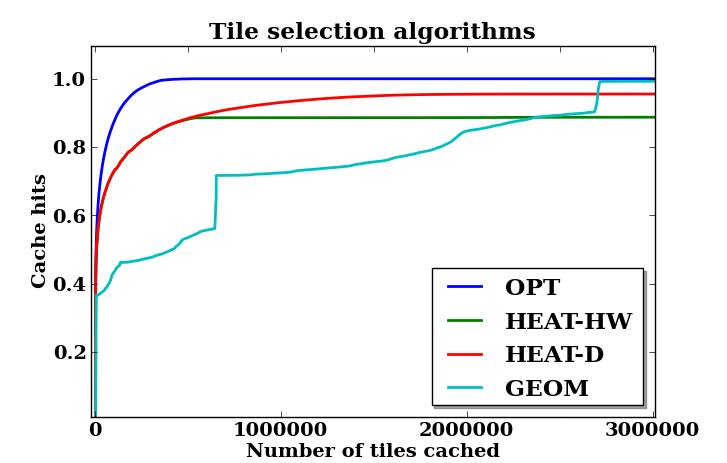
\includegraphics[scale=0.4]{results_closeup2.png}
\caption{The performance of tile selection algorithms for the first 3 million tiles selected, using three days of training data. The result is averaged over several runs using different data sets.}
\label{fig:results}
\end{figure*}

In Figure \ref{fig:results}, we show the average hit ratios obtained by the algorithms we have developed for TileHeat, using the datasets described in Section \ref{sec:datasets}. 
The figure shows the hit ratio of the first three million tiles that are selected by the algorithms. A full materialization contains more than ten million tiles. OPT, however, has a $100\%$ hit ratio after selecting 500,000 tiles. 

%OPT has a $100\%$ hit ratio after selecting 500,000 tiles.  %We also compare our algorithms against GEOM, which is the tile selection algorithm currently used by KMS.
As mentioned previously, the throughput of materializing tiles has been measured by KMS to be $58$ tiles per second on their infrastructure. A time window of $7.2$ hours fits inside the low load time period from $10$ PM to $6$ AM. During this window, we can compute $1.5$ million tiles. Within this tile budget, our best algorithm, HEAT-D, achieves a hit ratio of $95\%$. GEOM achieves a hit ratio of $76\%$ within the same tile budget. The hit ratio of HEAT-D is thus $25\%$ better than GEOM for this tile budget.

In general, we see that our algorithms rise significantly faster towards high hit ratios for small sets of tiles, e.g., in the 500,000 tile range. It is also clear that HEAT-D outperforms HEAT-HW after 500,000 tiles, and overall dominates HEAT-HW. This is because HEAT-D ranks more tiles than HEAT-HW, i.e., by ranking tiles that are not requested in the training workloads. We conclude that the additional tiles boost the hit ratio significantly, which confirms our hypothesis that tiles that are near to each other have similar access frequencies.

At around $2.6$ million tiles, GEOM overtakes HEAT-D, and becomes optimal. A peculiar effect of GEOM is a staircase effect that can be seen in Figure~\ref{fig:results}. We believe that this is an artifact of the way GEOM selects tiles --- selecting row-by-row the tiles that intersect the geometries provided. At certain latitudes, the rows cross over highly popular areas like the capital of Denmark, Copenhagen. The city of Copenhagen is clearly visible as a high-heat, dark area in the right side of each of the heatmaps shown in Figure~\ref{fig:heatmaps}. There are several steps in the staircase, as this effect is repeated at higher resolutions.

